% TEMPLATE AND PACKAGES ----------------------------------------------------------------------------

\documentclass[sigplan, nonacm, screen]{acmart}

% Packages for plotting
\usepackage{chngpage}
\usepackage{pgfplots}
\usepgfplotslibrary{groupplots}

\usepackage[dvipsnames]{xcolor}

% PLOT HELPERS -------------------------------------------------------------------------------------

% Process statistics for plots
\immediate\write18{data/statistics.sh}

\begin{document}

% TITLE, AUTHORS, ABSTRACT AND KEYWORDS ------------------------------------------------------------

\title{Tuning and Profiling LAMMPS on Deucalion}

\author{Humberto Gomes}
\email{pg59806@alunos.uminho.pt}
\affiliation{
    \institution{University of Minho}
    \city{Braga}
    \country{Portugal}
}

\author{José Lopes}
\email{pg59807@alunos.uminho.pt}
\affiliation{
    \institution{University of Minho}
    \city{Braga}
    \country{Portugal}
}

\begin{abstract} % ---------------------------------------------------------------------------------

    Molecular dynamics simulations with LAMMPS can be computationally demanding, requiring efficient
    use of modern High-Performance Computing (HPC) resources. This paper presents a performance
    study and tuning of LAMMPS on the ARM partition of the Deucalion supercomputer. We
    systematically assess the impact of parallelism type, core count, checkpointing strategy, and
    interconnect selection using the LJ and Rhodo benchmarks. Our results demonstrate that a
    NUMA-aware MPI+OpenMP configuration achieves a 10.8\,\% performance improvement over a naïve
    MPI-only approach. Profiling reveals additional optimization opportunities, such as compiler
    selection and MPI collective directives.

\end{abstract}

\maketitle

\section{Introduction} % ---------------------------------------------------------------------------
\label{introduction}

Molecular dynamics (MD) simulations enable the study of material properties, biological processes,
and chemical reactions at the atomic scale. LAMMPS \cite{lammps} is a widely used, open-source code
for performing such simulations. As simulations grow larger, requiring larger systems and longer
timescales, efficiently leveraging modern HPC resources becomes critical. Although these systems
offer substantial performance potential, realizing it usually requires careful application tuning.

This paper presents a performance study of LAMMPS on the ARM partition of the Deucalion
supercomputer \cite{deucalion}. We systematically tune various parameters on two benchmarks with
different computational profiles: the compute-bound LJ and the communication-intensive Rhodo,
scaling from 1 to 32 nodes. We then profile LAMMPS to identify further potential for optimization.

Our results show that a NUMA-aware MPI+OpenMP configuration yields the best performance. Profiling
identified potential future optimizations, such as the use of alternative compilers and collective
MPI directives.

\section{Background} % -----------------------------------------------------------------------------
\label{background}

\subsection{LAMMPS} % ------------------------------------------------------------------------------
\label{lammps}

LAMMPS (Large-scale Atomic/Molecular Massively Parallel Simulator) is an open-source classical MD
code, widely used for particle-based modeling of materials across various length scales, from atomic
and molecular to mesoscale and continuum levels \cite{lammps}.

At its core, LAMMPS integrates Newton's equations of motion for a system of interacting particles.
The forces between particles are derived from an interatomic potential, of which LAMMPS
supports a wide variety, ranging from inexpensive pairwise potentials, such as Lennard-Jones, to
computationally demanding manybody and machine-learning potentials. Long-range Coulombic
interactions are handled using FFT-based methods such as Particle-Particle Particle-Mesh (PPPM).

For parallel execution, LAMMPS employs a spatial decomposition strategy: the simulation domain is
partitioned into non-overlapping subdomains, each assigned to an MPI rank. Each rank stores its
own particles, as well as a halo of ghost particles of neighboring subdomains within the short-range
interaction cutoff distance. LAMMPS supports diverse domain decomposition strategies, from simple
uniform partitioning to complex adaptive strategies for improved load balancing on non-uniform
simulations, as shown in Figure \ref{lammps-partitioning}.

\vspace{-0.5\baselineskip}
\begin{figure}[h]
    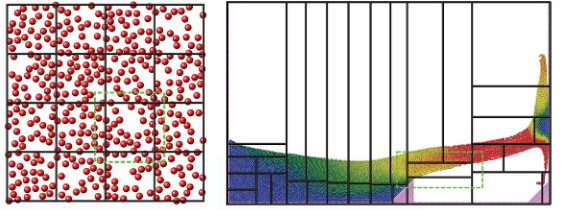
\includegraphics[width = 0.9\columnwidth]{res/Partitioning.png}
    \caption{
        LAMMPS orthogonal spatial decomposition -- uniform (left) and non-uniform (right)
        \cite{lammps}.
    }
    \label{lammps-partitioning}
\end{figure}
\vspace{-0.5\baselineskip}

Each timestep involves advancing the positions of the particles, communicating ghost particle data
with neighboring ranks, rebuilding Verlet-style neighbor lists (if necessary), computing short-range
forces and, optionally, using FFT-based solvers for computing long-range interactions. Beyond MPI,
LAMMPS supports hybrid parallelism though accelerator packages that leverage thread-level or
Single-Instruction Multiple-Data (SIMD) parallelism for performance-critical kernels
\cite{lammps-accelerators}.

\subsection{Deucalion} % ---------------------------------------------------------------------------
\label{deucalion}

We conducted our work on the Deucalion supercomputer, a heterogeneous cluster comprising multiple
partitions with distinct node types \cite{deucalion}. Our experiments used the ARM partition, as it
usually offers higher availability, facilitating the allocation of large node counts.

Each ARM node is equipped with a Fujitsu A64FX CPU, an ARMv8.2-A processor with Scalable Vector
Extensions (SVE) support. Designed for HPC, the A64FX architecture, illustrated in Figure
\ref{a64fx-architecture}, comprises 48 cores at 2.0\,GHz, organized into four Core Memory Groups
(CMGs), with 12 cores per CMG. Memory access is non-uniform (NUMA), with each CMG connected to 
8\,GiB of High Bandwidth Memory (HBM), totaling 32\,GiB per node \cite{deucalion, a64fx-design}.

\begin{figure}[h]
    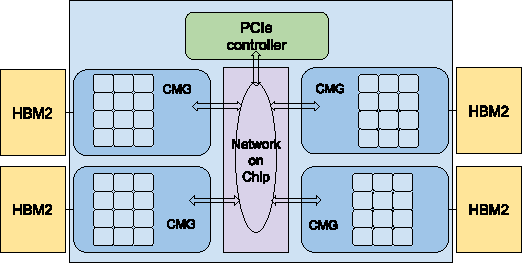
\includegraphics[width = 0.8\columnwidth]{res/A64FX.pdf}
    \caption{Architecture of the Fujitsu A64FX variant present on Deucalion \cite{a64fx-figure}.}
    \label{a64fx-architecture}
\end{figure}

Nodes within the same partition are interconnected via a 100\,Gb/s InfiniBand fat-tree network for
low-latency, high-bandwidth communication, as well as a 1\,Gb/s Ethernet network, mainly for
management purposes \cite{deucalion}.

For storage, each node includes a Western Digital CL SN720 512\,GB NVMe SSD. Additionally, all nodes
of all partitions are connected to a LustreFS Parallel File System (PFS) \cite{lustre}, which
employs a tiered storage architecture combining NVMe SSDs and HDDs. The PFS configuration includes 8
metadata nodes and 32 data nodes, delivering aggregate performance of 340\,GB/s for reads and
260\,GB/s for writes \cite{deucalion}.

\section{Benchmarks} % --------------------------------------------------------------------------
\label{benchmarks}

For benchmarking LAMMPS, we used two benchmarks with distinct computational characteristics
\cite{lammps-benchmarks}:

\begin{itemize}
    \item \textbf{LJ}: Simulates an atomic fluid, computing only short-range interactions using the
                       Lennard-Jones potential with a $2.5\,\sigma$ cutoff. The absence of
                       long-range interactions means the compute-bound pairwise force calculation
                       dominates this benchmark.

    \item \textbf{Rhodo}: Simulates the rhodopsin protein in a solvated lipid bilayer, using the
                          CHARMM force field with a 10\,\r{A} cutoff for short-range interactions.
                          Long-range Coulombic forces are handled via the PPPM method across compute
                          nodes, making this benchmark more sensitive to communication performance.
\end{itemize}

During our preliminary analysis, we found that both benchmarks completed in under one minute on a
single A64FX core, which was too short for meaningful multi-node scaling studies. To address this,
we scaled the simulation axes to increase the number of atoms, thereby extending the runtime.
However, large axis scales led to out-of-memory (OoM) errors, preventing single-node execution and
thus full strong scaling analyses. Consequently, we selected the maximum supported axis scale and
increased the number of iterations to further extend the runtimes to approximately 30 minutes on a
single node. The final benchmark configurations are presented in Table
\ref{benchmark-configurations}.

\begin{table}[h]
    \caption{Final configuration of LAMMPS benchmarks.}
    \label{benchmark-configurations}

    \begin{tabular}{lrrr}
        \toprule
        Benchmark & Axes Scale &   Atoms & Iterations \\
        \midrule
        LJ        &         13 & 70.3\,M &        500 \\
        Rhodo     &          5 &    4\,M &        500 \\
        \bottomrule
    \end{tabular}
\end{table}

% TODO - é preciso "running on Rocky Linux 8.5 (kernel 4.18.0-348.23.1.el8\_5)"?

All tests were conducted on the ARM partition of the Deucalion supercomputer, using LAMMPS
\mbox{2024-08-29}, as provided by Deucalion's environment modules. This version was compiled using
GCC 13.3.0 \cite{gcc}, and uses OpenMPI 5.0.3 \cite{open-mpi} for inter-process communication.

\section{Tuning} % ---------------------------------------------------------------------------------
\label{tuning}

\subsection{Methodology} % -------------------------------------------------------------------------
\label{tuning-methodology}

To maximize LAMMPS' performance, we employed a cascading optimization approach, adjusting one
variable at a time and selecting the best-performing configuration before proceeding to the next.
While this method significantly reduces the number of required measurements, it may converge only to
a local, rather than global, performance optimum.

For each variable, we conducted a strong scaling analysis for both benchmarks to assess LAMMPS'
performance across different node counts. For each node count, we recorded LAMMPS' self-reported
throughput, as well as its per-task runtime breakdown, which we then used to analyze the results. We
performed only one run per node count, acknowledging that this approach is susceptible to outlier
measurements. However, this was necessary to stay within our allotted compute hours on Deucalion. We
remain confident in the reliability of our results, as preliminary testing showed high consistency:
the maximum deviation across repeated measurements for the same configuration was just 1.9\,\%.

We tuned the following variables in the specified order:

\begin{itemize}
    \item \textbf{Parallelism type}: On CPUs, LAMMPS supports distributed-memory parallelism via
                                     MPI, as well as hybrid parallelism, by combining MPI with
                                     either OpenMP or Kokkos \cite{lammps-accelerators}. Our goal
                                     was to determine whether any parallelism type offers a
                                     performance advantage, and whether hybrid parallelism could
                                     benefit from NUMA awareness, for example, by running one MPI
                                     rank per NUMA node instead of per compute node.

    \item \textbf{Core count}: As a compute-bound application, LAMMPS typically scales efficiently
                               and can leverage high core counts. However, system services and
                               OpenMPI background threads may delay the scheduling of LAMMPS'
                               threads, potentially degrading overall performance. We hypothesize
                               that reserving a few threads for these tasks may improve performance.

    \item \textbf{Checkpointing strategy}: We introduced periodic checkpointing to disk in the LJ
                                           and Rhodo benchmarks to evaluate its impact on
                                           application performance. We also explored whether this
                                           impact can be mitigated by sharding checkpoint data
                                           across multiple files (e.g., one file per MPI rank) or
                                           through more complex schemes, such as tiering node-local
                                           storage and the PFS
                                           \cite{tiered-llm-checkpointing, hacc}.

    \item \textbf{Interconnect}: For pedagogical reasons, we assessed the importance of
                                 high-performance interconnects in HPC clusters by comparing LAMMPS'
                                 performance using Infiniband, IP over Infiniband (\texttt{IPoIB})
                                 and Ethernet.
\end{itemize}

\subsection{Parallelism Type} % --------------------------------------------------------------------
\label{tuning-parallelism-type}

To compare distributed-memory and hybrid parallelism, we evaluated the following configurations,
each using the maximum number of threads / processes supported, matching the number of cores per
node:

\begin{itemize}
    \item \texttt{MPI}: Each compute node runs multiple MPI ranks, one per core, up to 48 processes
                        per node;

    \item \texttt{OMP}: Each compute node runs a single MPI rank, which spawns up to 48 OpenMP
                        threads;

    \item \texttt{OMP-NUMA}: Each compute node runs four MPI ranks, one for each NUMA node, with
                             each spawning up to 12 OpenMP threads;

    \item \texttt{KOKKOS} and \texttt{KOKKOS-NUMA}: Similar to \texttt{OMP} and \texttt{OMP-NUMA},
                                                    respectively, but using Kokkos instead of OpenMP
                                                    for thread parallelism \cite{kokkos}. These
                                                    configurations are incompatible with the Rhodo
                                                    benchmark.
\end{itemize}

Our results are presented in Figure \ref{parallelism-plot}. For the LJ benchmark, all configurations
except \texttt{KOKKOS} exhibit linear scaling, with performance differences between them arising
only from variations in single-node performance. In constrast, Rhodo, which is more dependent on
inter-process communication, does not scale linearly. For example, at 32 nodes using the
\texttt{OMP-NUMA} configuration, each MPI rank spends on average 29.14\,\% of its time in
communication tasks (e.g., synchronizing atoms across ranks or computing long-range interactions), a
value which increases with the node count. For LJ, the time in communication-bound tasks is much
lower, only 13.6\,\%.

\begin{figure}[h]
    \input{plots/parallelism.tex}
    \caption{
        Strong scaling of the LJ and Rhodo benchmarks using different parallelism configurations.
    }
    \label{parallelism-plot}
\end{figure}

Across both benchmarks and all node counts, \texttt{OMP-NUMA} consistently delivers the best
performance. At 32 nodes in the LJ benchmark, it yields a 10.8\,\% performance advantage over a
naïve MPI configuration and a 190.8\% improvement over the worst-performing configuration
(\texttt{KOKKOS}). Since LAMMPS parallelism backends are implemented differently from each other,
it is impossible to isolate a single factor responsible for the observed performance differences.
However, LAMMPS per-task timing breakdowns provide a partial justification: \texttt{OMP-NUMA}
requires the least time to compute short-range interactions, the most time-consuming task in both
benchmarks.

Note that some datapoints for certain parallelism configurations at lower node counts are missing.
These configurations resulted in OoM errors, as OpenMP and Kokkos may duplicate data to ensure
thread-safe operation \cite{lammps-slides}. Thus, while some configurations might offer better
performance, they may be infeasible due to memory constraints.

\subsection{Core Count} % --------------------------------------------------------------------------
\label{tuning-core-count}

Next, we ran LAMMPS using 44 threads per compute node (11 per NUMA node) to investigate whether
leaving unallocated cores for system tasks and OpenMPI background threads could improve performance.
The results are presented in Figure \ref{cores-plot}.

\begin{figure}[h]
    \begin{tikzpicture}
    \begin{groupplot}[
        % Group two plots
        group style = {
            group size        = 1 by 2,
            vertical sep      = 0 cm,
            x descriptions at = edge bottom
        },
        % Plot dimensions
        width  = 0.95\columnwidth,
        height = 4.2cm,
        % Axes styling
        xlabel             = {\# Nodes},
        x tick label style = {font = \scriptsize},
        y tick label style = {font = \scriptsize},
        xlabel near ticks,
        ylabel near ticks,
        % X axis range
        xmin = 0,
        xmax = 33,
        % Grid
        xtick       = {1, 2, 4, 8, 16, 32},
        xmajorgrids = true,
        ymajorgrids = true,
        grid style  = {
            dashed,
            gray!80
        }
    ]

        % Top panel
        \nextgroupplot [
            % Label styles
            y label style = {font = \small, align = center},
            % Y axis
            ylabel = {\textbf{LJ} \\ \footnotesize Rel. throughput},
            ymin   = 0.91,
            ymax   = 1.09,
            % Legend
            legend to name    = parallelism,
            legend cell align = left,
            legend style      = {
                at                                    = {(0.5, 1.05)},
                anchor                                = south,
                legend columns                        = 2,
                font                                  = \small,
                /tikz/every even column/.append style = {column sep = 1ex}
            }
        ]

        \addplot+ [mark = none, black, very thick] coordinates {(1, 1) (32, 1)};

        \addplot+ [
            thick,
            red!80!black,
            mark      = +,
            mark size = 2.5pt
        ] table [
            x       = NNODES,
            y       = REL_THROUGHPUT,
            col sep = comma
        ] {data/cores/LJ.csv};

        \legend{48 Threads, 44 Threads};

        % Bottom panel
        \nextgroupplot [
            % Label styles
            x label style = {font = \small},
            y label style = {font = \small, align = center},
            % Y axis
            ylabel = {\textbf{Rhodo} \\ \footnotesize Rel. throughput},
            ymin   = 0.91,
            ymax   = 1.09
        ]

        \addplot+ [mark = none, black, very thick] coordinates {(1, 1) (32, 1)};

        \addplot+ [
            thick,
            red!80!black,
            mark      = +,
            mark size = 2.5pt
        ] table [
            x       = NNODES,
            y       = REL_THROUGHPUT,
            col sep = comma
        ] {data/cores/RHODO.csv};
    \end{groupplot}

    \node[anchor = south, yshift = 1pt] at (group c1r1.north) {
        \pgfplotslegendfromname{parallelism}
    };
\end{tikzpicture}

    \caption{
        LJ and Rhodos throughput with 44 threads relative to 48 threads, across different node
        counts.
    }
    \label{cores-plot}
    \vspace{-2\baselineskip}
\end{figure}

For both benchmarks, performance was generally worse with the lower thread count. However, the
performance gap between the configurations narrowed as the node count increased, with the 44-thread
configuration even outperforming the 48-thread one for Rhodo on 32 nodes.

An analysis of LAMMPS' per-task time breakdown revealed that this was due to reduced time spent on
communication tasks. While close-range force calculations were faster with 48 threads (due to
greater arithmetic capacity), communication, where the 44-thread configuration excelled, became a
more significant portion of both benchmarks' total wall time as the node count increased.
Consequently, the performance gap between the two configurations diminished.

Given the overall superior performance of the 48-thread configuration, we used this setup for all
subsequent tests. Nevertheless, for node counts exceeding 32, it may be worthwhile to re-evaluate
lower thread-count configurations.

\subsection{Checkpointing Strategy} % --------------------------------------------------------------
\label{tuning-checkpointing-strategy}

Checkpointing --- periodically saving the simulation state to persistent storage --- is essential
for fault tolerance, as it allows for progress recovery in the event of a failure. In our
benchmarks, we implemented full simulation checkpointing every 100 iterations using LAMMPS'
\texttt{dump} command \cite{lammps-dump}. At higher node counts, this frequency results in a
checkpoint being created every few seconds. While this rate is excessive, it generates an intensive
PFS workload, making it easier to distinguish performance differences between checkpointing
configurations, of which we tested the following:

\begin{itemize}
    \item \texttt{NOSTORAGE}: No checkpointing is performed;

    \item \texttt{LOCAL}: Each MPI rank writes a checkpoint file to its node's local NVMe storage.
                          This scenario represents the best-case performance for applications that
                          store checkpoints locally before asynchronously copying them to the PFS
                          \cite{tiered-llm-checkpointing, hacc};

    \item \texttt{PFS-SHARDED}: Each MPI rank writes a checkpoint file directly to the PFS;

    \item \texttt{PFS-SINGLE}: All MPI ranks write to a shared checkpoint file on the PFS.
\end{itemize}

Our results are presented in Figure \ref{storage-plot}.

\begin{figure}[h]
    \input{plots/storage.tex}
    \caption{
        LJ and Rhodos throughput across different node counts and checkpointing techniques (relative
        to no checkpointing).
    }
    \label{storage-plot}
\end{figure}

We observe that \texttt{LOCAL} and \texttt{PFS-SHARDED} checkpointing introduce little to no
performance degradation. In contrast, \texttt{PFS-SINGLE} exhibits a distinct behavior: in the LJ
benchmark with 32 nodes, checkpointing accounts for, on average, 6.35\,\% of rank execution time,
compared to only 0.18\,\% for \texttt{PFS-SHARDED}. Straggler ranks, as evidenced by a very high
standard deviation in I/O time (119.6\,\%), further delay checkpointing, resulting in a 13.0\,\%
throughput reduction for \texttt{PFS-SINGLE} in relation to \texttt{NOSTORAGE}. The effect is less
pronounced in Rhodo due to the smaller checkpoint size (914\,MiB \emph{vs.} 16\,GiB). For subsequent
tests, checkpointing will remain disabled.

\subsection{Interconnect} % ------------------------------------------------------------------------
\label{tuning-interconnect}

Finally, we compared the performance of LAMMPS using Infiniband, \texttt{IPoIB}, and Ethernet.
Theoretical bandwidth and latency measurements, obtained via the OSU MPI benchmarks \cite{osu},
are presented in Table \ref{osu-results}. These results reveal differences of up to $104\times$ in
bandwidth and $17\times$ in latency among the interconnects.

\begin{table}[h]
    \caption{Unidirectonal bandwidth and ping-pong latency of the interconnects tested.}
    \label{osu-results}

    \begin{tabular}{lrr}
        \toprule
        Interconnect   &  Bandwidth (MB/s) & Latency ($\mu$s) \\
        \midrule
        Infiniband     &         12 298.6 &                 2.85 \\
        \texttt{IPoIB} &          1 515.0 &                39.17 \\
        Ethernet       &            117.5 &                48.55 \\
        \bottomrule
    \end{tabular}
\end{table}

We then evaluated how these theoretical differences affect LAMMPS performance. Our results are
presented in Figure \ref{interconnect-plot}.

\begin{figure}[h]
    \begin{adjustwidth}{-1cm}{-1cm}
        \centering
        \begin{tikzpicture}
    \begin{groupplot}[
        % Group two plots
        group style = {
            group size        = 1 by 2,
            vertical sep      = 0 cm,
            x descriptions at = edge bottom
        },
        % Plot dimensions
        width  = 0.95\columnwidth,
        height = 4.2cm,
        % Axes styling
        xlabel             = {\# Nodes},
        x tick label style = {font = \scriptsize},
        y tick label style = {font = \scriptsize},
        xlabel near ticks,
        ylabel near ticks,
        % X axis range
        xmin = 0,
        xmax = 33,
        % Grid
        xtick       = {1, 2, 4, 8, 16, 32},
        xmajorgrids = true,
        ymajorgrids = true,
        grid style  = {
            dashed,
            gray!80
        }
    ]

        % Top panel
        \nextgroupplot [
            % Label styles
            y label style = {font = \small, align = center},
            % Y axis
            ylabel = {\textbf{LJ} \\ \footnotesize Throughput (it/s)},
            ymin   = 0,
            ymax   = 9.99,
            % Legend
            legend to name    = parallelism,
            legend cell align = left,
            legend style      = {
                at                                    = {(0.5, 1.05)},
                anchor                                = south,
                legend columns                        = 4,
                font                                  = \small,
                /tikz/every even column/.append style = {column sep = 1ex}
            }
        ]

        \addplot+ [
            thick,
            red!80!black,
            mark      = x,
            mark size = 2.5pt
        ] table [
            x       = NNODES,
            y       = THROUGHPUT,
            col sep = comma
        ] {data/network/LJ-INFINIBAND.csv};

        \addplot+ [
            thick,
            ForestGreen,
            mark      = +,
            mark size = 2.5pt
        ] table [
            x       = NNODES,
            y       = THROUGHPUT,
            col sep = comma
        ] {data/network/LJ-IPoIB.csv};

        \addplot+ [
            thick,
            blue!80!black,
            mark      = Mercedes star,
            mark size = 2.5pt
        ] table [
            x       = NNODES,
            y       = THROUGHPUT,
            col sep = comma
        ] {data/network/LJ-ETHERNET.csv};

        \addplot [mark = none, black, thick, dotted] coordinates {(1, 0.275) (32, 8.8)};

        \legend{Infiniband, \texttt{IPoIB}, Ethernet, \textnormal{Linear}};

        % Bottom panel
        \nextgroupplot [
            % Label styles
            x label style = {font = \small},
            y label style = {font = \small, align = center},
            % Y axis
            ylabel = {\textbf{Rhodo} \\ \footnotesize Throughput (it/s)},
            ymin   = 0,
            ymax   = 9.99,
            ytick  = {0, 2, 4, 6, 8, 10}
        ]

        \addplot+ [
            thick,
            red!80!black,
            mark      = x,
            mark size = 2.5pt
        ] table [
            x       = NNODES,
            y       = THROUGHPUT,
            col sep = comma
        ] {data/network/LJ-INFINIBAND.csv};

        \addplot+ [
            thick,
            ForestGreen,
            mark      = +,
            mark size = 2.5pt
        ] table [
            x       = NNODES,
            y       = THROUGHPUT,
            col sep = comma
        ] {data/network/LJ-IPoIB.csv};

        \addplot+ [
            thick,
            blue!80!black,
            mark      = Mercedes star,
            mark size = 2.5pt
        ] table [
            x       = NNODES,
            y       = THROUGHPUT,
            col sep = comma
        ] {data/network/LJ-ETHERNET.csv};

        \addplot [mark = none, black, thick, dotted] coordinates {(1, 0.275) (32, 10.24)};
    \end{groupplot}

    \node[anchor = south, yshift = 1pt] at (group c1r1.north) {
        \pgfplotslegendfromname{parallelism}
    };
\end{tikzpicture}

    \end{adjustwidth}
    \caption{Strong scaling of the LJ and Rhodo benchmarks using different interconnects.}
    \label{interconnect-plot}
\end{figure}

Our analysis shows negligible performance differences between Infiniband and IPoIB. However, when
using Ethernet, both benchmarks become communication-bound, resulting in poor scalability. For
32-node runs, LAMMPS' runtime breakdowns indicate that, compared to Infiniband, a node running the
LJ benchmark spends, on average, 70.37\,\% of its time on communication tasks (\emph{vs.}
13.61\,\%), while the Rhodo benchmark spends, on average, 75.35\,\% (\emph{vs.} 29.14\,\%). This
leads to performance degradations of 65.6\,\% (LJ) and 77.4\,\% (Rhodo) at 32 nodes. This phenomenon
is explored in greater detail in Section \ref{profiling-interconnect}.

% TODO - mistral

In summary, optimal LAMMPS performance is achieved using the \texttt{OMP-NUMA} parallelism
configuration, with 48 LAMMPS threads per compute node and the Infiniband interconnect. Future tests
will be performed without checkpointing, but if properly configured (e.g., by using sharding),
checkpointing does not harm performance at the scale and frequency tested.


\section{Profiling} % ------------------------------------------------------------------------------
\label{profiling}

\subsection{Methodology} % -------------------------------------------------------------------------
\label{profiling-methodology}

Following tuning, we profiled LAMMPS to identify the root causes of the previous results and to
explore potential configuration adjustments for further optimization. Our profiling focused on the
following questions:

\begin{itemize}
    \item Could performance be further improved by replacing libraries (e.g., BLAS) with
          A64FX-optimized versions?
    \item What communication patterns dominate LAMMPS, and how do they scale with node count? Is
          there evidence of load imbalance?
    \item How does MPI communication performance compare between Ethernet and Infiniband?
\end{itemize}

To answer these questions, we profiled three configurations of the Rhodo benchmark: 1-node and
32-node setups in their optimal configurations, and a 32-node setup with Ethernet instead of
Infiniband. We used NVIDIA NSight Systems 25.1a \cite{nvidia-nsight} to trace MPI calls and sample
regular function calls.

\subsection{Profiling Overhead} % ------------------------------------------------------------------
\label{profiling-overhead}

During preliminary testing, we observed significant profiling overhead, as shown in Figure
\ref{overhead-plot}.

\begin{figure}[h]
    \input{plots/overhead.tex}
    \caption{
        Runtimes of the Rhodo benchmark (total and long-range interaction calculations)
        relative to their non-profiled equivalents, across different node counts.
    }
    \label{overhead-plot}
\end{figure}

The minimum profiling overhead obeserved was 8.2\,\% for a single node. However, for 32 nodes,
profiling increased LAMMPS' self-reported execution time fourfold! Analysis of LAMMPS' per-task
runtime breakdowns revealed that most of the overhead originated from the \linebreak[4]
communication-bound long-range force calculations, \linebreak[4] which, for 32 nodes, were
$12.7\times$ slower when profiled.

To mitigate this overhead, we tested the following approaches in isolation: disabling MPI tracing,
disabling function call sampling, and profiling only one MPI rank per compute node. However, these
adjustments yielded negligible improvements in an 8-node configuration. Ideally, we would have
adopted lightweight profilers such as mpiP for MPI tracing \cite{mpip} and \texttt{perf record}
\cite{perf} for function call sampling, but time constraints prevented their implementation.
Therefore, we replaced our 32-node tests with 8-node tests, limiting overhead to 19.7\,\%.

\subsection{Further Optimization Potential} % ------------------------------------------------------
\label{profiling-further-optimization-potential}

To identify kernels with potential for further optimization, we analyzed the call graph of the first
MPI rank in a single-node run. The dominant hotspot is the \linebreak[4]
\texttt{PairLJCharmmCoulLongOMP::compute} kernel, which consumes $62.51\%$ of CPU time. This kernel,
responsible for computing short-range forces at each timestep, is highly compute-bound. Thus, it
could benefit from optimizations such as more efficient code generation using alternative compilers
\cite{optimizing-lammps}, or a manual rewrite to leverage ARM SVE instructions for SIMD processing.
For comparison, the INTEL package enables SIMD processing on x86 processors and has demonstrated
$2\times$ speedups in previous work \cite{lammps-slides}.

While no other kernel emerged as an immediate candidate for optimization, we also evaluated external
libraries for potential replacement with more efficient alternatives. For instance, FFTW
\cite{fftw}, used in long-range force computations, could be substituted with Fujitsu's A64FX-tuned
FFTW implementation \cite{fj-fftw}. However, the expected performance gains would be minimal, as the
FFTW kernel accounts for only 0.44\,\% of total CPU usage in the profiled configuration.

\subsection{MPI Communication Breakdown} % ---------------------------------------------------------
\label{profiling-mpi}

Next, we analyzed the MPI communication patterns of LAMMPS, comparing single-node and 8-node
configurations. Tables \ref{mpi-single-node} and \ref{mpi-multi-node} report the time share of each
of each MPI directive in relation to total communication time and overall application wall time.

\begin{table}[h]
    \caption{MPI directive time on the $1$-node configuration.}
    \label{mpi-single-node}

    \begin{tabular}{lrr}
        \toprule
        MPI Directive           & MPI Time (\%) & Wall Time (\%) \\
        \midrule
        \texttt{MPI\_Wait}      &          41.0 &           1.32 \\
        \texttt{MPI\_Allreduce} &          31.0 &           1.01 \\
        \texttt{MPI\_Send}      &          21.0 &           0.68 \\
        Others                  &           7.0 &             -- \\
        \bottomrule
    \end{tabular}
\end{table}

\begin{table}[h]
    \caption{MPI directive time on the $8$-node configuration.}
    \label{mpi-multi-node}

    \begin{tabular}{lrr}
        \toprule
        MPI Directive           & MPI Time (\%) & Wall Time (\%) \\
        \midrule
        \texttt{MPI\_Wait}      &          41.0 &           7.69 \\
        \texttt{MPI\_Allreduce} &          28.0 &           5.30 \\
        \texttt{MPI\_Send}      &          16.0 &           2.98 \\
        \texttt{MPI\_Waitany}   &           7.0 &           1.45 \\
        Others                  &           8.0 &             -- \\
        \bottomrule
    \end{tabular}
\end{table}

The distribution of communication time across MPI primitives is consistent between configurations:
both are dominated by time spent waiting for messages and performing all-reductions. However, with
8 nodes, waiting becomes even more pronounced, with the \texttt{MPI\_Waitany} directive also
contributing significantly. Despite the similar breakdown of communication types, the overall
communication time increases substantially with node count, accounting for 17.87\,\% of wall time in
the 8-node configuration compared to 3.08\,\% in the single-node case. This trend is expected, as
multi-node setups require additional synchronization and, unlike the single-node case, use
Infiniband rather than shared memory.

Additionally, we observed evidence of load imbalance, which arises because different MPI ranks
process varying numbers of atoms. A profiler timeline analysis revealed that straggler nodes delayed
progress at synchronization barriers. LAMMPS' internal instrumentation further confirmed this,
showing performance disparities of up to 25.1\,\% between the slowest and fastest MPI ranks in the
8-node configuration. There are also indications of load imbalance among OpenMP threads, with up to
5.9\,\% of CPU time spent in OpenMP spinlock barriers. However, this metric may not accurately
reflect the true imbalance, as cores can idle in these barriers, halting sampling. Unfortunately, we
were unable to configure the profiler to correctly trace OpenMP events.

One potential optimization to reduce communication overhead is to replace node-to-node messaging
with collective MPI directives in the PPPM long-range interaction calculation \cite{kspace-modify}.

\subsection{Interconnect} % ------------------------------------------------------------------------
\label{profiling-interconnect}

Finally, we evaluated the impact of replacing Infiniband with Ethernet in an 8-node configuration.
The resulting MPI directive breakdown is presented in Table \ref{mpi-multi-node-ethernet}. As
expected, performance degraded significantly: every directive accounts for a substantially larger
fraction of wall time compared to the Infiniband configuration (Table \ref{mpi-multi-node}), and MPI
communication now consumes 75.7\% of the total runtime.

\begin{table}[h]
    \caption{MPI directive time on a $8$-node Ethernet configuration.}
    \label{mpi-multi-node-ethernet}

    \begin{tabular}{lrr}
        \toprule
        MPI Directive           & MPI Time (\%) & Wall Time (\%) \\
        \midrule
        \texttt{MPI\_Send}      &          58.0 &          44.70 \\
        \texttt{MPI\_Waitany}   &          25.0 &          19.60 \\
        \texttt{MPI\_Wait}      &          12.0 &           9.21 \\
        \texttt{MPI\_Allreduce} &           2.0 &           2.19 \\
        Others                  &           3.0 &             -- \\
        \bottomrule
    \end{tabular}
\end{table}

The most notable change is the dramatic increase in \texttt{MPI\_Send} time, which now dominates the
runtime. This shift indicates a bandwidth-limited configuration, as Ethernet's bandwidth is
$104\times$ lower than that of Infiniband. These results highlight the critical role of
high-performance interconnects in HPC clusters.

\section{Conclusion} % -----------------------------------------------------------------------------
\label{conclusion}

In this paper, we optimized LAMMPS' configuration for best performance on Deucalion's ARM partition.
By employing hybrid MPI+OpenMP NUMA-aware parallelism, we achieved performance improvements of up to
10.8\,\% over a naïve MPI configuration. We also demonstrated that sharding can eliminate the
performance overhead of simulation checkpointing, and that interconnect performance can become a
bottleneck, even for compute-bound applications like LAMMPS. Finally, through profiling, we
identified potential optimizations for future work, including enabling collective MPI directives,
exploring alternative compilers, or extending LAMMPS to support SIMD parallelism on the A64FX via
SVE instructions.

\begin{acks} % -------------------------------------------------------------------------------------

    This work made use of compute hours awarded by grant 2025.00010.HPCVLAB.UMINHO, funded by the
    Foundation for Science and Technology (FCT).
\end{acks}

% BIBLIOGRAPHY -------------------------------------------------------------------------------------

\bibliographystyle{ACM-Reference-Format}
\bibliography{references}

\end{document}
